\section{Part II: Improving Convergence}

In Part I, basic SGD shows instability near the optimum, with accuracy fluctuating between 96\%--98\%. This highlights the need to improve convergence and enable more stable and effective fine-tuning near the optimum.

\subsection{Hyper-Parameter Analysis}

In order to systematically investigate the convergence behavior of SGD, this experiment varies two key hyper-parameters: learning rate and batch size. The selected ranges are: \textbf{Learning Rates:} \( \eta = 0.1, 0.01, 0.001 \) and \textbf{Batch Sizes:} \( m = 1, 10, 100 \).

\subsubsection{Results and Discussion}

\begin{figure}[h]
    \centering
    \begin{minipage}[b]{0.45\textwidth}
        \centering
        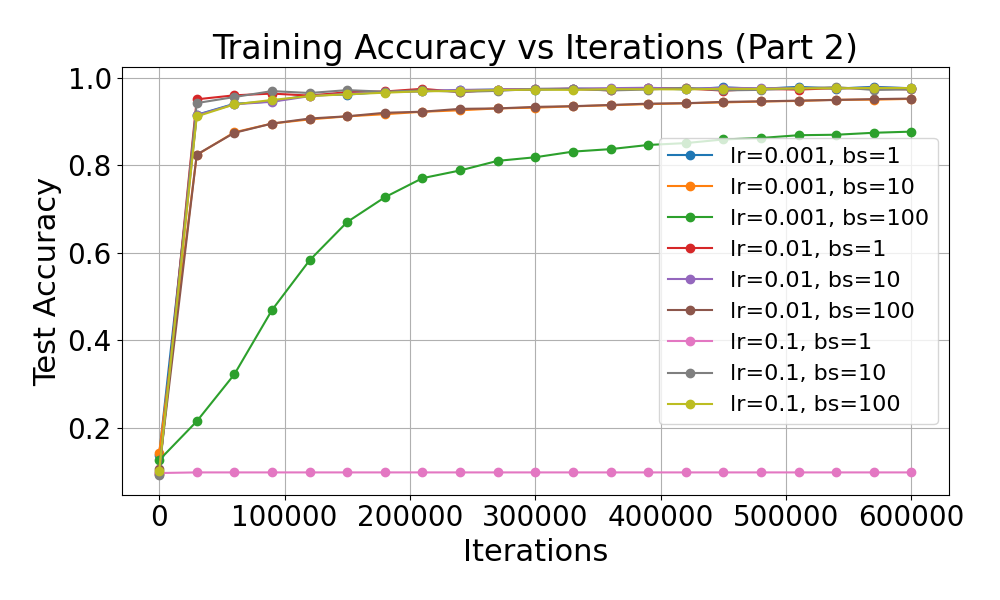
\includegraphics[width=\linewidth]{../data/part2/accuracy_training_plot}
        \caption{Accuracy across Iterations.}
        \label{fig:training}
    \end{minipage}
    \hfill
    \begin{minipage}[b]{0.45\textwidth}
        \centering
        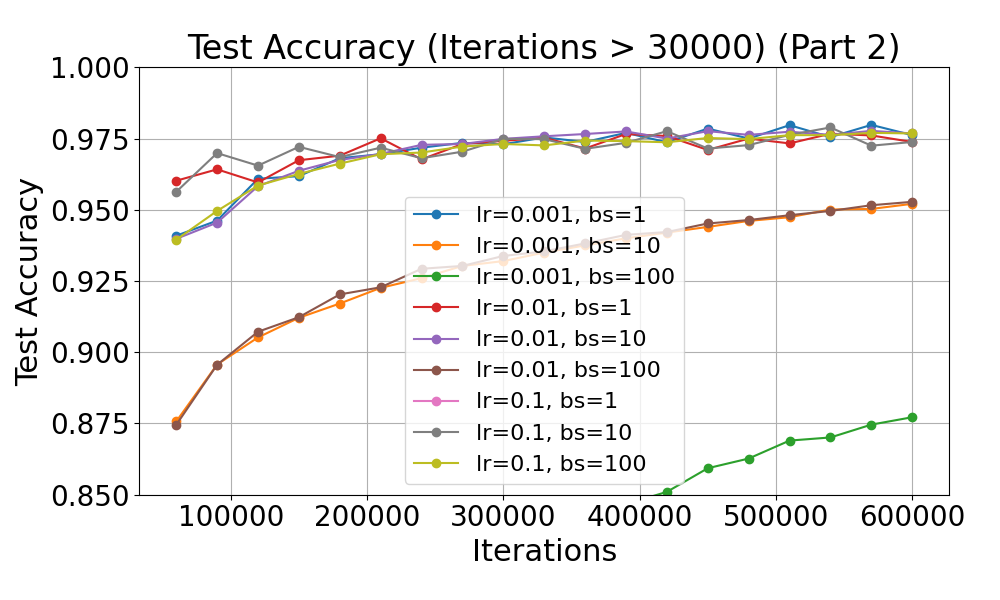
\includegraphics[width=\linewidth]{../data/part2/accuracy_after30000}
        \caption{Accuracy after 30000 Iterations.}
        \label{fig:30000}
    \end{minipage}
\end{figure}

\begin{wraptable}{r}{0.46\textwidth}
    \centering
    \begin{tabular}{|c|c|c|c|c|}
        \hline
        \textbf{\(\eta\)} & \textbf{\(m\)} & \textbf{Loss} & \textbf{Accuracy} & \textbf{Time (s)} \\
        \hline
        0.1   & 1   & 2.3026 & 0.0980  & 589 \\
        0.1   & 10  & 0.0253 & 0.9774  & 555 \\
        0.1   & 100 & 0.0161 & 0.9768  & 544 \\
        0.01  & 1   & 0.0253 & 0.9738  & 588 \\
        0.01  & 10  & 0.0167 & 0.9769  & 551 \\
        0.01  & 100 & 0.1591 & 0.9528  & 547 \\
        0.001 & 1   & 0.0166 & 0.9762  & 591 \\
        0.001 & 10  & 0.1603 & 0.9521  & 558 \\
        0.001 & 100 & 0.4820 & 0.8772  & 546 \\
        \hline
    \end{tabular}
    \caption{Final performance metrics at epoch 10}
    \label{tab:learning_rate_batch_size}
\end{wraptable}

Figures~\ref{fig:training} and~\ref{fig:30000} illustrated the training accuracy over iterations and a more detailed view of the accuracy after 30,000 iterations, respectively. The Table~\ref{tab:learning_rate_batch_size} summarizes the performance metrics for different combinations of learning rates and batch sizes.

Notably, when using a learning rate of 0.1 with a batch size of 1, the model records an extremely low accuracy (9.8\%). In contrast, increasing the batch size to 10 or 100 with the same learning rate leads to significant improvements: the loss reduces to approximately 0.0253 and 0.0161, while accuracy reaches around 97.7\%. These configurations also slightly reduce computation time, suggesting that larger batch sizes not only stabilize learning but also enhance computational efficiency.

Meanwhile, Smaller learning rates (e.g., 0.001) produce smoother curves as each update nudges the weights more gently. Similarly, larger batch sizes (e.g., 100) average out noise across more samples, reducing gradient variance and stabilizing the learning trajectory. Conversely, larger learning rates (e.g., 0.1) introduce oscillations, which are also observed with small batch sizes (e.g., 1).

Moreover, pairing lower learning rates with a batch size of 100 yields higher losses (0.1591 for \(\eta\)=0.01 and 0.4820 for \(\eta\)=0.001) and a reduction in accuracy (roughly 95.3\% and 87.7\%, respectively). Combined with the plots, they indicate that the training process has not yet been given sufficient iterations to fully converge.

The optimal configuration in these experiments appears to be a high learning rate (0.1) combined with a large batch size (100), which achieves enough rapid convergence with a smooth trajectory and high overall accuracy, while managing computational time effectively.



\subsection{Learning Rate Decay}

A high initial learning rate can accelerate convergence by allowing the optimizer to take large steps, but it may hinder fine-tuning as the optimum is approached. When near a minimum, maintaining a high learning rate risks overshooting the optimum and could cause oscillations rather than convergence. To address this issue, it is common to gradually reduce the learning rate—a process known as learning rate decay. This reduction allows the optimisation algorithm to take smaller, more precise steps during the later stages of training, effectively fine-tuning the parameters as the loss landscape flattens near the optimum~\cite{you2019how}.

\subsubsection{Learning Rate Decay Implementation}
In the implementation, the learning rate is linearly interpolated from an initial value \(\eta_{\mathrm{init}} = 0.1\) to a predefined final value \(\eta_{\mathrm{final}} = 10^{-4}\).

At the end of each epoch, the current epoch counter is incremented. When learning rate decay is enabled, the decay parameter \(\alpha\) is computed as the ratio of the current epoch number to the total number of epochs:
\[
    \alpha = \frac{k}{N},
\]
where \(k\) is the current epoch and \(N\) is the total number of epochs.

Using this decay parameter, the learning rate for the next epoch is updated using the following formula:
\[
    \eta_k = \eta_0 (1 - \alpha) + \alpha \eta_N,
\]
where \(\eta_0\) is the initial learning rate, \(\eta_N\) is the final learning rate, \(\eta_k\) is the learning rate at epoch.


\subsubsection{Results and Discussion}
\begin{figure}[h]
    \centering
    \begin{minipage}[b]{0.45\textwidth}
        \centering
        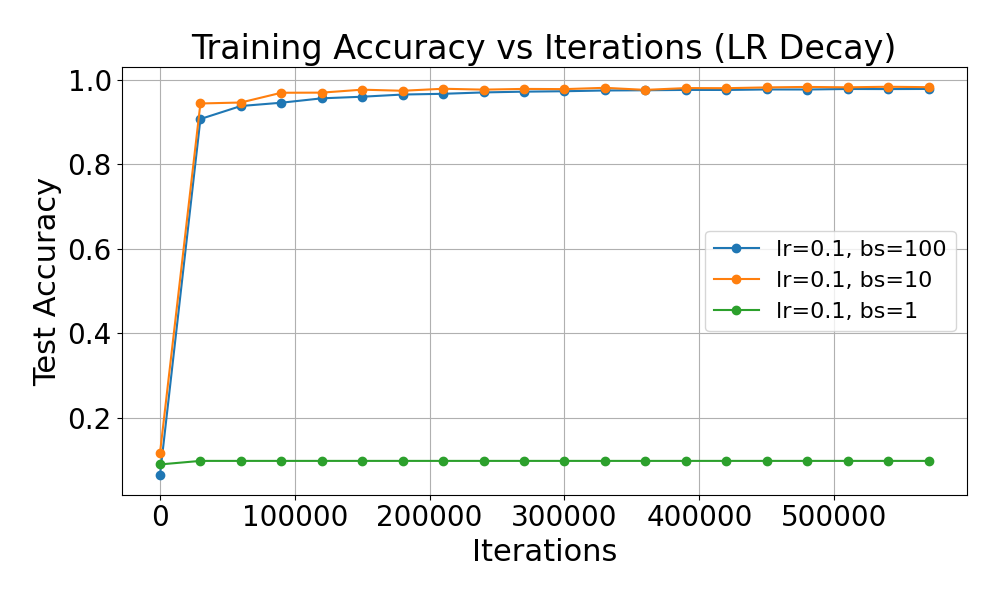
\includegraphics[width=\linewidth]{../data/part2/learning_rate_decay/accuracy_training_plot_lr_decay}
        \caption{Accuracy across Iterations with Learning Rate Decay.}
        \label{fig:training_lr_decay}
    \end{minipage}
    \hfill
    \begin{minipage}[b]{0.45\textwidth}
        \centering
        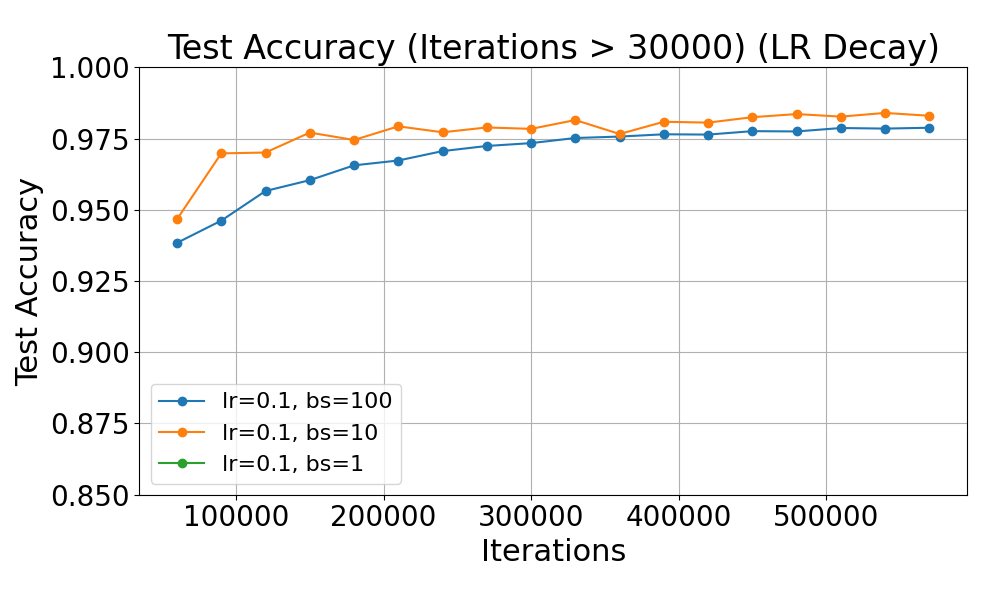
\includegraphics[width=\linewidth]{../data/part2/learning_rate_decay/accuracy_after_30000_plot_lr_decay}
        \caption{Accuracy after 30000 Iterations with Learning Rate Decay.}
        \label{fig:30000_lr_decay}
    \end{minipage}
\end{figure}

\begin{wraptable}{r}{0.38\textwidth}
    \centering
    \begin{tabular}{|c|c|c|c|c|}
        \hline
        \textbf{\(\eta_0\)} & \textbf{\(\eta_N\)} & \textbf{\(m\)} & \textbf{Loss} & \textbf{Accuracy} \\
        \hline
        0.1   & 0.0001   & 1 & 2.3026  & 0.0980 \\
        0.1   & 0.0001  & 10 & 0.0017  & 0.9827 \\
        0.1   & 0.0001 & 100 & 0.0311  & 0.9788 \\
        \hline
    \end{tabular}
    \caption{Performance metrics at epoch 10 with learning rate decay.}
    \label{tab:learning_rate_decay}
\end{wraptable}

For Figures~\ref{fig:training_lr_decay},~\ref{fig:30000_lr_decay}, and Table~\ref{tab:learning_rate_decay}, several important observations regarding the effect of learning rate decay can be drawn. First, the configuration employing a batch size of 1—whether with a decayed learning rate from 0.1 to 0.001 or with a constant learning rate of 0.1—consistently results in very low accuracy (9.8\%).

In contrast, the configurations with larger batch sizes (10 and 100) display improvements in performance, comparing when no learning rate decay employed. Specifically, the configuration with a batch size of 10 achieves an accuracy of 98.30\% (from 97.74\%) with a loss of 0.0020, while the batch size of 100 yields an accuracy of 97.88\% (from 97.68\%) and a loss of 0.0311. The smoother training accuracy curves observed in these cases indicate that learning rate decay contributes to more gradual and stable convergence.

\subsection{Momentum}

Momentum is a technique designed to accelerate convergence and mitigate oscillations during optimization by incorporating an exponentially decaying moving average of past gradients~\cite{fu2023when}. By accumulating a history of gradient information, momentum helps the optimizer maintain consistent update directions, thereby smoothing the updates and enabling the algorithm to overcome small local minima.

\subsubsection{Momentum Implementation}

In implementation, momentum is incorporated through an additional velocity term \(v\) associated with each weight parameter \(w\). The update rule for momentum is formulated as follows:

\[
    v = \alpha\, v - \eta \frac{1}{m}\sum_{i=1}^{m} \nabla L_i(x_i, w)
\]
\[
    w = w + v
\]

where \(\eta\) represents the learning rate, \(m\) is the batch size, \(\nabla L_i(x_i, w)\) is the gradient of the loss with respect to the weight \(w\) for the \(i\)-th training example in the batch, \(\alpha\) is the momentum coefficient.

The previous velocity is scaled by the momentum coefficient \(\alpha\) and then decreased by the current gradient (averaged over the batch and scaled by the learning rate \(\eta\)). The computed velocity \(v\) is then added to the corresponding weight \(w\), effectively smoothing the weight updates and promoting faster convergence.

\subsubsection{Results and Discussion}

\begin{figure}[h]
    \centering
    \begin{minipage}[b]{0.45\textwidth}
        \centering
        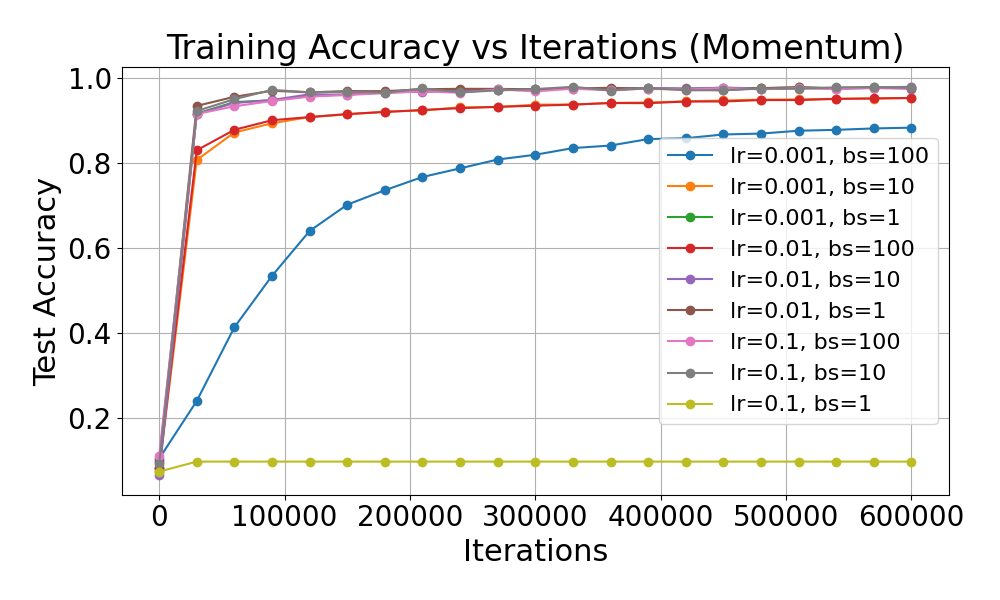
\includegraphics[width=\linewidth]{../data/part2/momentum/accuracy_training_plot_momentum}
        \caption{Accuracy across Iterations with Momentum.}
        \label{fig:training_momentum}
    \end{minipage}
    \hfill
    \begin{minipage}[b]{0.45\textwidth}
        \centering
        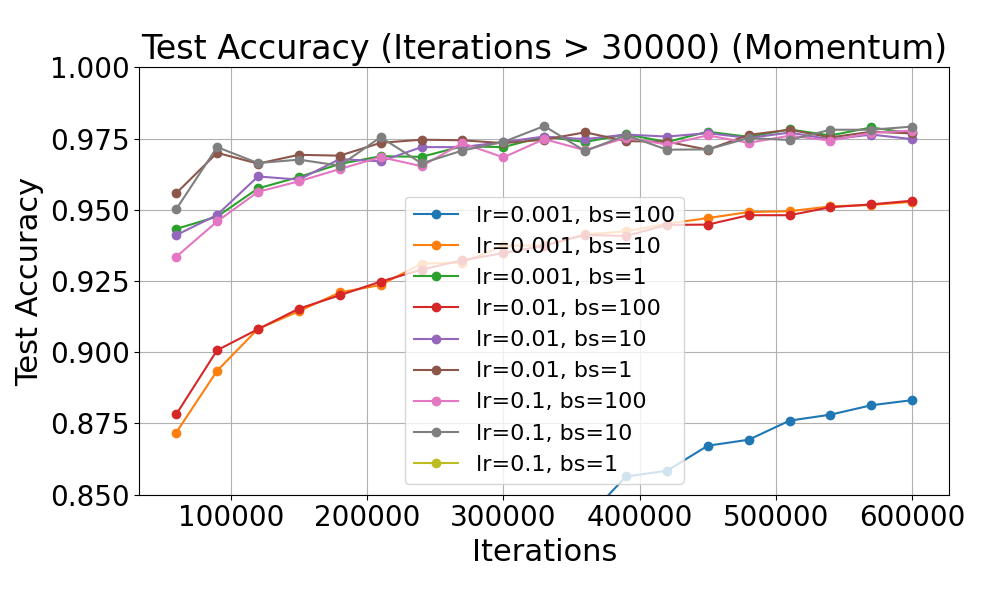
\includegraphics[width=\linewidth]{../data/part2/momentum/accuracy_training_plot_momentum_post_30000}
        \caption{Accuracy after 30000 Iterations with Momentum.}
        \label{fig:30000_momentum}
    \end{minipage}
\end{figure}

\begin{wraptable}{r}{0.38\textwidth}
    \centering
    \begin{tabular}{|c|c|c|c|c|}
        \hline
        \textbf{\(\alpha\)} & \textbf{\(\eta\)} & \textbf{\(m\)} & \textbf{Loss} & \textbf{Accuracy} \\
        \hline
        0.1   & 0.1   & 1 & 2.3026  & 0.0980 \\
        0.1   & 0.1  & 10 & 0.0250  & 0.9792 \\
        0.1   & 0.1 & 100 & 0.0136  & 0.9778 \\
        0.1   & 0.01  & 1 & 0.0272  & 0.9768 \\
        0.1   & 0.01  & 10 & 0.0145  & 0.9748 \\
        0.1   & 0.01 & 100 & 0.1630  & 0.9532 \\
        0.1   & 0.001 & 1 & 0.0145  & 0.9768 \\
        0.1   & 0.001 & 10 & 0.1487 & 0.9528 \\
        0.1   & 0.001 & 100 & 0.4821 & 0.8772 \\
        \hline
    \end{tabular}
    \caption{Performance metrics at epoch 10 with momentum.}
    \label{tab:momentum}
\end{wraptable}

In Figures~\ref{fig:training_momentum},~\ref{fig:30000_momentum}, and Table~\ref{tab:momentum}, several key observations can be drawn. Notably, regardless of whether momentum is applied, the configuration with a batch size of 1 and a learning rate of 0.1 again produces very low accuracy (9.8\%). In contrast, all other configurations exhibit a slight improvement in accuracy compared to previous experiments without momentum, and their accuracy curves are slightly smoother. These findings support that a momentum coefficient of 0.1 is a sensible choice, and employing momentum can help to stabilize the training process.

\subsection{Combined Techniques: Learning Rate Decay with Momentum}

Integrating learning rate decay with momentum might leverage the strengths of both approaches. Learning rate decay adapts the step size during training, grained updates when close to convergence. Concurrently, momentum incorporates a moving average of past gradients, which smooths the update trajectory and helps in surmounting shallow local minima or flat regions. The fusion of these techniques allows the optimizer to maintain directionality and stability, even as the step size diminishes, thereby reducing oscillations and overshooting near the minimum.

\subsubsection{Results and Discussion}

\begin{figure}[h]
    \centering
    \begin{minipage}[b]{0.45\textwidth}
        \centering
        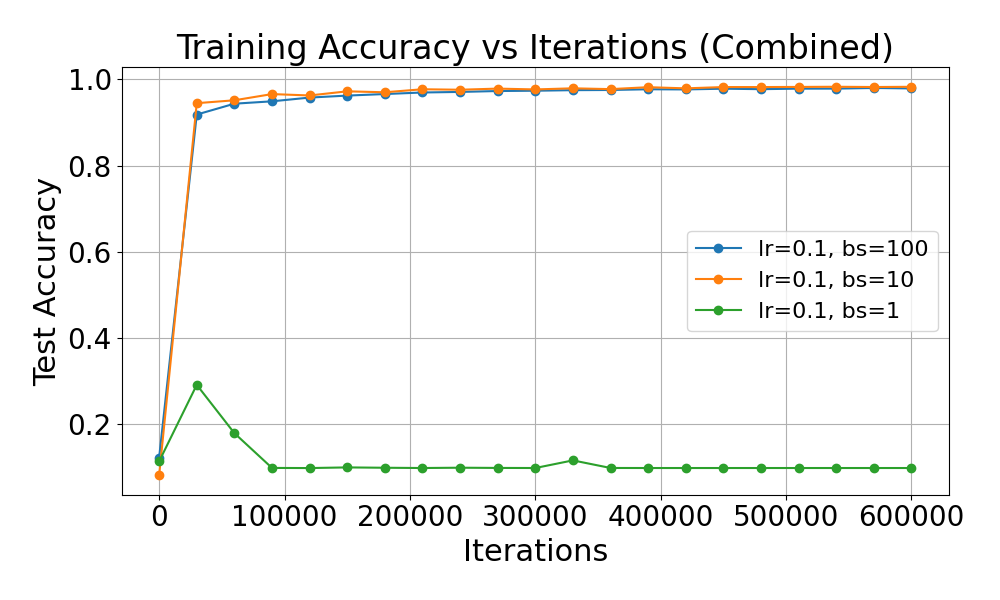
\includegraphics[width=\linewidth]{../data/part2/combined/accuracy_training_plot_combined}
        \caption{Accuracy across Iterations with Combined Techniques.}
        \label{fig:training_combined}
    \end{minipage}
    \hfill
    \begin{minipage}[b]{0.45\textwidth}
        \centering
        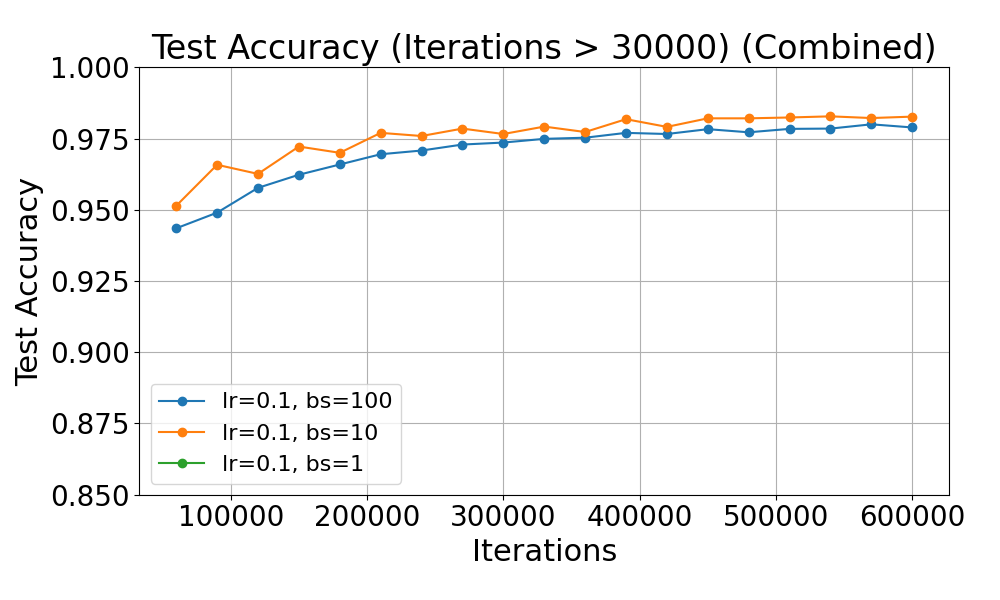
\includegraphics[width=\linewidth]{../data/part2/combined/accuracy_training_plot_combined_post_30000}
        \caption{Accuracy after 30000 Iterations with Combined Techniques.}
        \label{fig:30000_combined}
    \end{minipage}
\end{figure}

\begin{wraptable}{r}{0.46\textwidth}
    \centering
    \begin{tabular}{|c|c|c|c|c|c|}
        \hline
        \textbf{\(\alpha\)} & \textbf{\(\eta_0\)} & \textbf{\(\eta_N\)} & \textbf{\(m\)} & \textbf{Loss} & \textbf{Accuracy} \\
        \hline
        0.1 & 0.1  & 0.0001   & 1 & 2.3026  & 0.0980 \\
        0.1 & 0.1  & 0.0001  & 10 & 0.0016  & 0.9828 \\
        0.1 & 0.1  & 0.0001 & 100 & 0.0271  & 0.9789 \\
        \hline
    \end{tabular}
    \caption{Performance metrics at epoch 10 with combined techniques.}
    \label{tab:combination}
\end{wraptable}

Figures~\ref{fig:training_combined},~\ref{fig:30000_combined}, and Table~\ref{tab:combination} demonstrate an improvement over previous experimental configurations. Notably, the configuration that yielded the highest performance—achieving 98.28\% accuracy and a minimum loss of 0.0016—was obtained with a batch size of 10, an initial learning rate of 0.1 decaying to a final learning rate of 0.0001, and a momentum coefficient of 0.1. This optimal setting effectively balances rapid early convergence with the fine-tuning capabilities required in later stages of training, underscoring the benefits of integrating learning rate decay with momentum.